% DO NOT COMPILE THIS FILE DIRECTLY!
% This is included by the other .tex files.

\begin{frame}{What is ELF?}
    \begin{itemize}
        \item ELF stands for Executable and Linkable Format\footnote{\url{https://refspecs.linuxfoundation.org/elf/elf.pdf}}.
        \item It is a common standard file format for executables, object code, shared libraries, and core dumps.
        \item Originally developed by Unix System Laboratories and now widely used in Unix-like operating systems.
    \end{itemize}
\end{frame}

\begin{frame}{Structure of an ELF File}
    \begin{itemize}
        \item An ELF file consists of three main parts:
        \begin{itemize}
            \item \textbf{Header:} Contains metadata about the file type, architecture, and entry point.
            \item \textbf{Program Header Table:} Describes how the file should be loaded into memory.
            \item \textbf{Section Header Table:} Provides information about the sections in the file.
        \end{itemize}
        \item ELF files are designed to be flexible and extensible.
    \end{itemize}
\end{frame}

\begin{frame}{Benefits of ELF}
    \begin{itemize}
        \item Platform-independent format, enabling portability.
        \item Simplifies the linking and loading process.
        \item Supports dynamic linking, reducing redundancy.
        \item Extensively used in modern development environments.
    \end{itemize}
\end{frame}

\begin{frame}[fragile]
\frametitle{Binwalk Output}

\begin{lstlisting}[language=bash, basicstyle=\ttfamily, breaklines=true]
Sample: 6420f5d7d48b75d687b8356e93c82721bb536c633d773f8985f74c8977425f04

binwalk sample
\end{lstlisting}

\begin{tabular}{ccp{0.6\textwidth}}
\textbf{Decimal} & \textbf{Hexadecimal} & \textbf{Description}\\
0                & 0x0                  & ELF, 32-bit LSB executable, Intel 80386, version 1 (SYSV) \\
13111            & 0x3337               & Boot section Start 0x58028941 End 0x5A41 \\
13115            & 0x333B               & Boot section Start 0x5A41 End 0x0 \\
\end{tabular}

\vspace{1cm}

$\to$ matched signatures
\end{frame}

\begin{frame}[fragile]
\frametitle{Using Binwalk}
\framesubtitle{Sample: 9e70725640c4284e2049e4b25c9cc46cca496053cebf69855ec25acc9bd63e05}
\begin{tabular}{|c|c|p{0.6\textwidth}|}
\hline
\textbf{Decimal} & \textbf{Hexadecimal} & \textbf{Description} \\ \hline
0                & 0x0                  & ELF, 64-bit LSB executable, AMD x86-64, version 1 (GNU/Linux) \\ \hline
600864           & 0x92B20              & Unix path: /usr/share/locale \\ \hline
612774           & 0x959A6              & Unix path: /usr/lib/getconf \\ \hline
620336           & 0x97730              & Unix path: /usr/lib/locale \\ \hline
622368           & 0x97F20              & Unix path: /usr/lib/locale/locale-archive \\ \hline
674903           & 0xA4C57              & Unix path: /usr/lib/x86\_64-linux-gnu/ \\ \hline

\textbf{778039}           & \textbf{0xBDF37}              & \textbf{mcrypt 2.2 encrypted data, algorithm: blowfish-448, mode: CBC, keymode: 8bit} \\ \hline
\end{tabular}

\end{frame}

\begin{frame}
\frametitle{Using Binwalk}

\begin{itemize}
    \item \textbf{Encrypted Data:}
    \begin{itemize}
        \item The file contains data encrypted using \textbf{mcrypt 2.2}.
    \end{itemize}
    \item \textbf{Encryption Algorithm:}
    \begin{itemize}
        \item Algorithm: \textbf{Blowfish-448}, a symmetric block cipher with a 448-bit key size.
    \end{itemize}
    \item \textbf{Cipher Mode:}
    \begin{itemize}
        \item Mode: \textbf{CBC (Cipher Block Chaining)} for enhanced security via block interdependency.
    \end{itemize}
    \item \textbf{Key Mode:}
    \begin{itemize}
        \item Key processed in \textbf{8-bit mode}, possibly a default for mcrypt configurations.
    \end{itemize}
    \item \textbf{Implications:}
    \begin{itemize}
        \item Decryption requires the encryption key and potentially an initialization vector (IV).
        \item Indicates sensitive or protected data within the file.
        \item Poses a reverse engineering challenge without the key.
    \end{itemize}
\end{itemize}

\end{frame}

\begin{frame}[fragile]
\frametitle{Extracting the content}
Sample: 9e70725640c4284e2049e4b25c9cc46cca496053cebf69855ec25acc9bd63e05
\begin{lstlisting}[language=bash, basicstyle=\ttfamily, frame=single, breaklines=true]
dd if=sample of=extracted_data bs=1 skip=778039
\end{lstlisting}

\begin{itemize}
    \item Binwalk uses signatures to identify and extract data from files.
    \item Determine the size of the detected block for further analysis.
    \item Evaluate whether the detection is a false positive by inspecting the data manually or using additional tools.
\end{itemize}

\end{frame}


\begin{frame}[fragile]
\frametitle{ELF Symbols from Binary Analysis}

Extract symbols from binary excluding GBLIBC references

Sample: 6420f5d7d48b75d687b8356e93c82721bb536c633d773f8985f74c8977425f04
\begin{lstlisting}[language=bash, basicstyle=\ttfamily, frame=single]
nm sample | grep -v GBLIBC
\end{lstlisting}


\begin{lstlisting}[basicstyle=\ttfamily, frame=single]
08048bfd t p4tch_sel1nux_codztegfaddczda
08048e9c t parse_cred
8050bb3 T prepare_fops_lsm_shellcode
08049215 t put_your_hands_up_hooker
0804b220 D r1ngrrrrrrr
0804988e t rey0y0code
0804b2c0 d ruujhdbgatrfe345
\end{lstlisting}
\end{frame}

\begin{frame}
\frametitle{ELF Symbols from Binary Analysis}

\begin{itemize}
    \item Interpretation of the output of tool \tt{nm}
    \item man page is your friend
\end{itemize}

\begin{tabular}{|c|p{0.7\textwidth}|}
\hline
\textbf{Symbol Type} & \textbf{Explanation} \\ \hline
a & The symbol's value is absolute and will not be changed by further linking. \\ \hline
b & The symbol is in the BSS data section. \\ \hline
d & The symbol is in the initialized data section. \\ \hline
r & The symbol is in the read-only data section. \\ \hline
t & The symbol is in the text (code) section. \\ \hline
w & The symbol is a weak symbol that has not been specifically tagged as a weak object symbol. \\ \hline
\end{tabular}

\end{frame}

\begin{frame}[fragile]
\frametitle{Using objdump to View ELF Sections}

\begin{lstlisting}[language=bash, basicstyle=\ttfamily, frame=single, breaklines=true]
objdump -h sample
\end{lstlisting}

\begin{itemize}
    \item \textbf{Output Structure:}
    \begin{itemize}
        \item Lists all sections in the ELF file, including their attributes.
        \item Provides information such as:
        \begin{itemize}
            \item \textbf{Idx}: Section index in the ELF file.
            \item \textbf{Name}: Name of the section (e.g., `.text`, `.data`).
            \item \textbf{Size}: Size of the section in bytes.
            \item \textbf{VMA (Virtual Memory Address)}: Where the section is loaded in memory.
            \item \textbf{File Off}: Offset of the section in the binary file.
            \item \textbf{Attributes}: Flags indicating section properties (e.g., `ALLOC`, `LOAD`, `READONLY`).
        \end{itemize}
    \end{itemize}
    \item \textbf{Use Case:}
    \begin{itemize}
        \item Identify key sections like `.text` (code), `.data` (initialized data), `.bss` (uninitialized data), and `.dtor` (destructors).
        \item Useful to identify the type of binary, such as a C program, C++, Go (Golang), etc. 
    \end{itemize}
\end{itemize}

\end{frame}



\begin{frame}[fragile]
\frametitle{ELF Section Details}

\begin{tabular}{clcccp{1cm}}
\textbf{Idx} & \textbf{Name}       & \textbf{Size}  & \textbf{VMA}     & \textbf{LMA}     & \textbf{File Off} \\
0            & .interp            & 00000013       & 08048134         & 08048134         & 00000134          \\
1            & .note.ABI-tag      & 00000020       & 08048148         & 08048148         & 00000148          \\
2            & .gnu.hash          & 00000030       & 08048168         & 08048168         & 00000168          \\
3            & .dynsym            & 00000290       & 08048198         & 08048198         & 00000198          \\
11           & .text              & 00001788       & 080489b0         & 080489b0         & 000009b0          \\

\end{tabular}

\vspace{1cm}

\begin{tabular}{cc}
\textbf{Idx} &  \textbf{Attributes}\\
0            &  CONTENTS, ALLOC, LOAD, READONLY, DATA \\
1            &  CONTENTS, ALLOC, LOAD, READONLY, DATA \\
2            &  CONTENTS, ALLOC, LOAD, READONLY, DATA \\
3            &  CONTENTS, ALLOC, LOAD, READONLY, DATA \\
11           &  CONTENTS, ALLOC, LOAD, READONLY, \textbf{CODE}
\end{tabular}

\end{frame}


\begin{frame}
\frametitle{Collaborative Malware Analysis Using MISP}

\centering
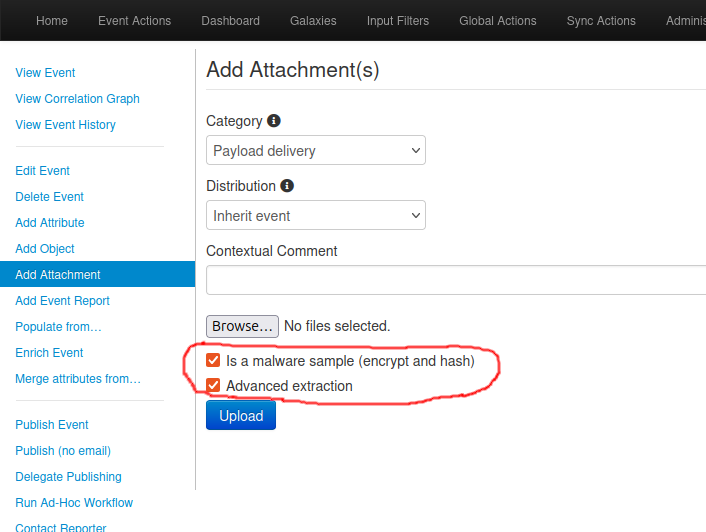
\includegraphics[width=0.8\textwidth]{img/upload2.png}

Uploading your sample to MISP

\end{frame}

\begin{frame}
\frametitle{Collaborative Malware Analysis Using MISP}

\centering
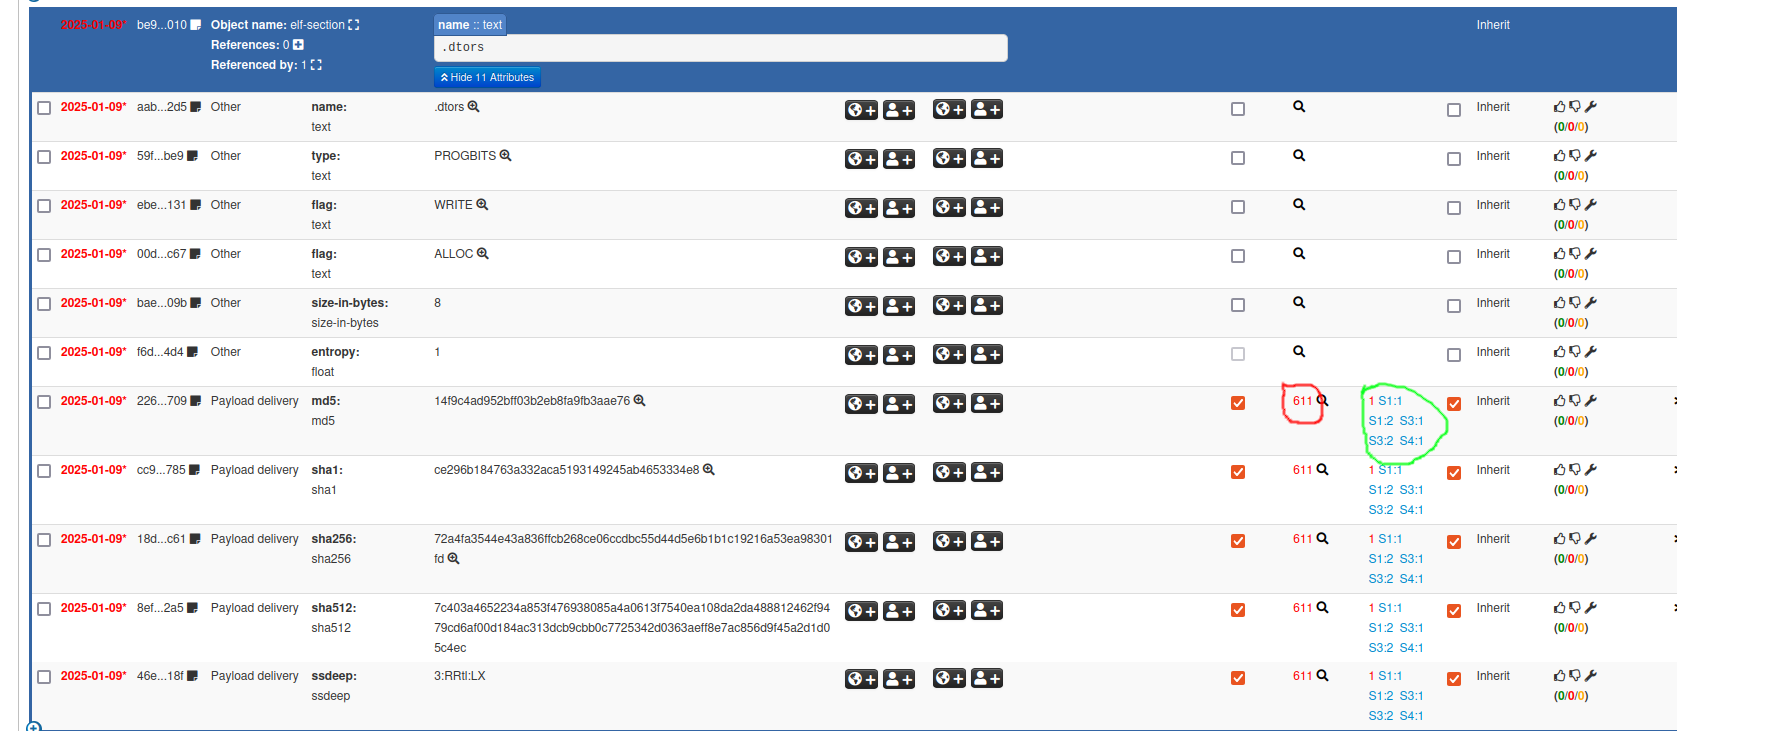
\includegraphics[width=0.8\textwidth]{img/correlation2.png}

\begin{itemize}
    \item Explore correlations between events and indicators.
    \item Analyze hits from threat intelligence feeds.
    \item Review hits from synchronization caches.
\end{itemize}

\end{frame}

\begin{frame}
\frametitle{Collaborative Malware Analysis Using MISP}

Exploring connected MISP instances within MISP-LEA

\centering
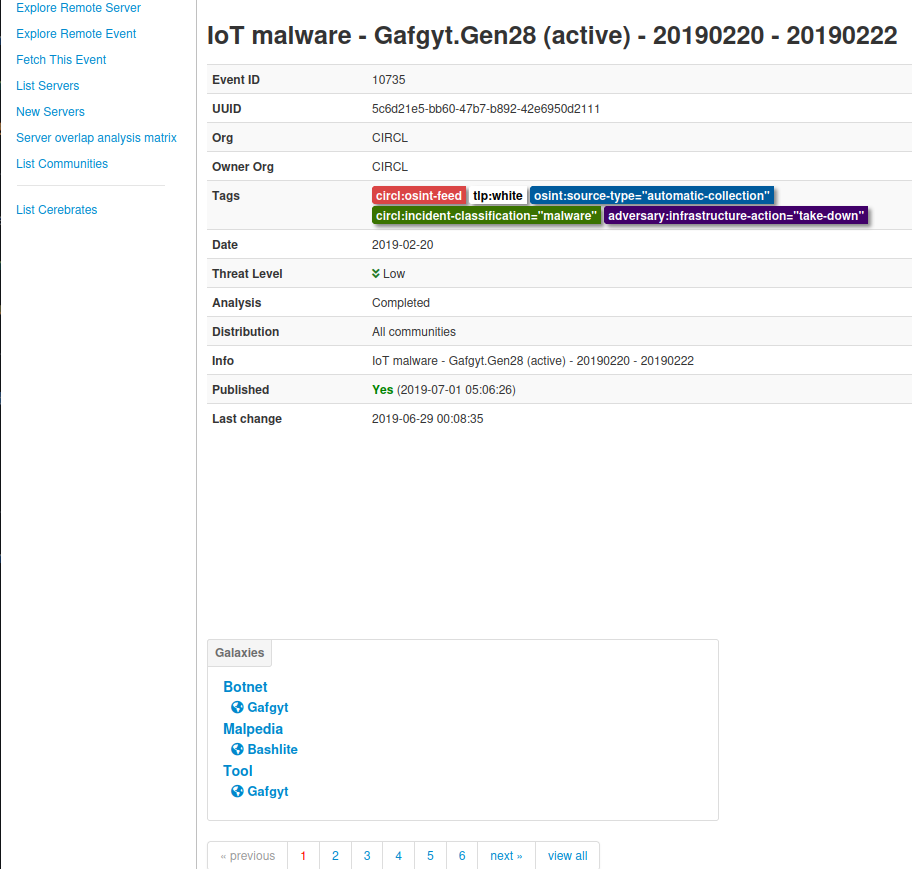
\includegraphics[width=0.6\textwidth]{img/foreign.png}

\end{frame}

\begin{frame}[fragile]
\frametitle{Disassembly of $<$main$>$ (Part 1) with objdump}

\begin{lstlisting}[basicstyle=\ttfamily\scriptsize]
8049d05 <main>:
 8049d05:       8d 4c 24 04             lea    0x4(%esp),%ecx
 8049d09:       83 e4 f0                and    $0xfffffff0,%esp
 8049d0c:       ff 71 fc                push   -0x4(%ecx)
 8049d0f:       55                      push   %ebp
 8049d10:       89 e5                   mov    %esp,%ebp
 8049d12:       51                      push   %ecx
 8049d13:       83 ec 34                sub    $0x34,%esp
 8049d16:       89 4d e4                mov    %ecx,-0x1c(%ebp)
 8049d19:       c7 04 24 cc a5 04 08    movl   $0x804a5cc,(%esp)
 8049d20:       e8 37 ec ff ff          call   804895c <puts@plt>
 8049d25:       e8 82 eb ff ff          call   80488ac <getuid@plt>
 8049d2a:       85 c0                   test   %eax,%eax
 8049d2c:       75 31                   jne    8049d5f <main+0x5a>
 8049d2e:       a1 20 b4 04 08          mov    0x804b420,%eax
 8049d33:       89 44 24 0c             mov    %eax,0xc(%esp)
 8049d37:       c7 44 24 08 1a 00 00    movl   $0x1a,0x8(%esp)
 8049d3e:       00
\end{lstlisting}

\end{frame}

% Slide 2
\begin{frame}[fragile]
\frametitle{Disassembly of $<$main$>$ (Part 2) with objdump}

\begin{lstlisting}[basicstyle=\ttfamily\scriptsize]
 8049d3f:       c7 44 24 04 01 00 00    movl   $0x1,0x4(%esp)
 8049d46:       00
 8049d47:       c7 04 24 42 a6 04 08    movl   $0x804a642,(%esp)
 8049d4e:       e8 89 eb ff ff          call   80488dc <fwrite@plt>
 8049d53:       c7 45 e8 01 00 00 00    movl   $0x1,-0x18(%ebp)
 8049d5a:       e9 1c 03 00 00          jmp    804a07b <main+0x376>
 8049d5f:       8b 55 e4                mov    -0x1c(%ebp),%edx
 8049d62:       8b 42 04                mov    0x4(%edx),%eax
 8049d65:       89 44 24 04             mov    %eax,0x4(%esp)
 8049d69:       8b 55 e4                mov    -0x1c(%ebp),%edx
 8049d6c:       8b 02                   mov    (%edx),%eax
 8049d6e:       89 04 24                mov    %eax,(%esp)
 8049d71:       e8 e2 f8 ff ff          call   8049658 <env_prepare>
 8049d76:       e8 59 fa ff ff          call   80497d4 <y0y0stack>
 8049d7b:       e8 b1 fa ff ff          call   8049831 <y0y0code>
\end{lstlisting}

\end{frame}



\begin{frame}
\frametitle{Introduction Ghidra}

\begin{itemize}
    \item \textbf{Disassembly and Decompilation:}
    \begin{itemize}
        \item Transforms binary code into human-readable assembly.
        \item Generates high-level language representations (C-like pseudocode).
    \end{itemize}
    \item \textbf{Cross-Platform Support:}
    \begin{itemize}
        \item Analyzes binaries for multiple architectures (x86, ARM, MIPS, etc.).
        \item Compatible with various operating systems (Windows, Linux, macOS).
    \end{itemize}
    \item \textbf{Collaboration:}
    \begin{itemize}
        \item Supports multi-user reverse engineering projects.
        \item Version-controlled changes for shared analysis.
    \end{itemize}
    \item \textbf{Scriptability:}
    \begin{itemize}
        \item Customize and automate analysis with Python and Java.
    \end{itemize}
    \item \textbf{Extensibility:}
    \begin{itemize}
        \item Add plugins and extend functionality for specific needs.
    \end{itemize}
    \item \textbf{Data Flow Analysis:}
    \begin{itemize}
        \item Tracks variables, functions, and references for better insight.
    \end{itemize}
\end{itemize}

\end{frame}

\begin{frame}
\frametitle{Static Analysis Using Ghidra}
\begin{itemize}
    \item Creating a project in Ghidra.
    \item Importing and analyzing a binary file.
\end{itemize}

\centering
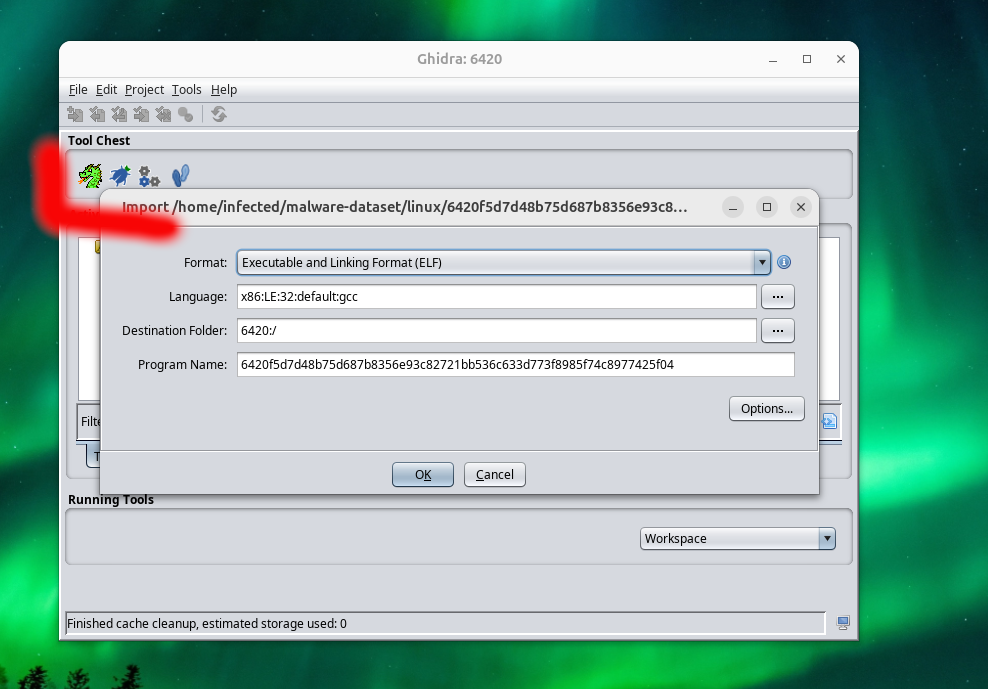
\includegraphics[width=0.6\textwidth]{img/g0.png}

\end{frame}

\begin{frame}
\frametitle{Static Analysis Using Ghidra}

\begin{itemize}
    \item Determine the type of binary (e.g., ELF, PE).
    \item Analyze the binary's metadata for key attributes such as architecture, endianness, and sections.
\end{itemize}

\centering
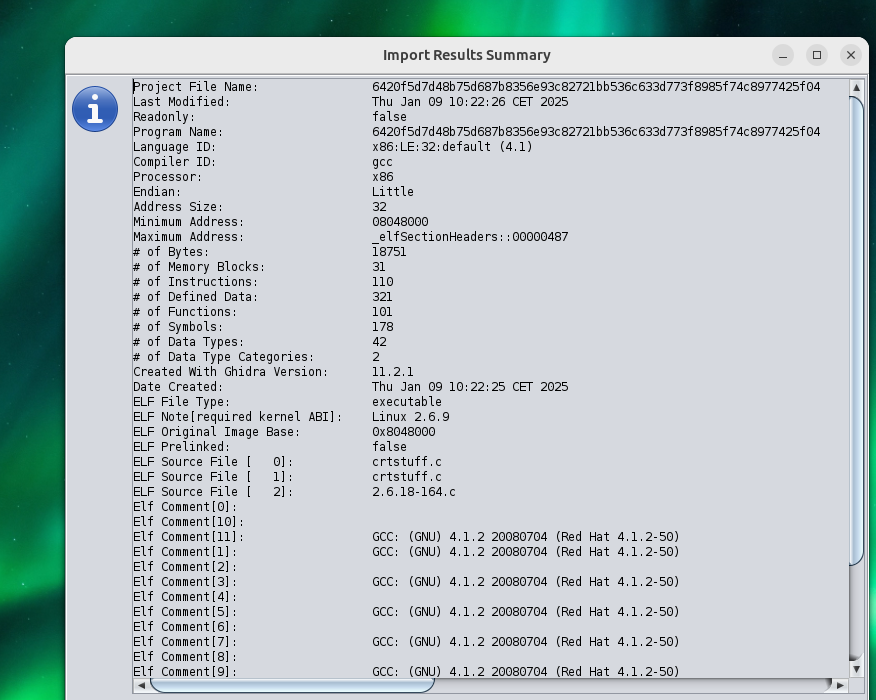
\includegraphics[width=0.6\textwidth]{img/g1.png}
\end{frame}

\begin{frame}
\frametitle{Static Analysis Using Ghidra}

\begin{itemize}
    \item Explore the functions defined within the binary.
    \item Analyze the disassembly view to examine low-level instructions.
    \item Utilize the decompiled view for a high-level representation of the code.
\end{itemize}

\centering
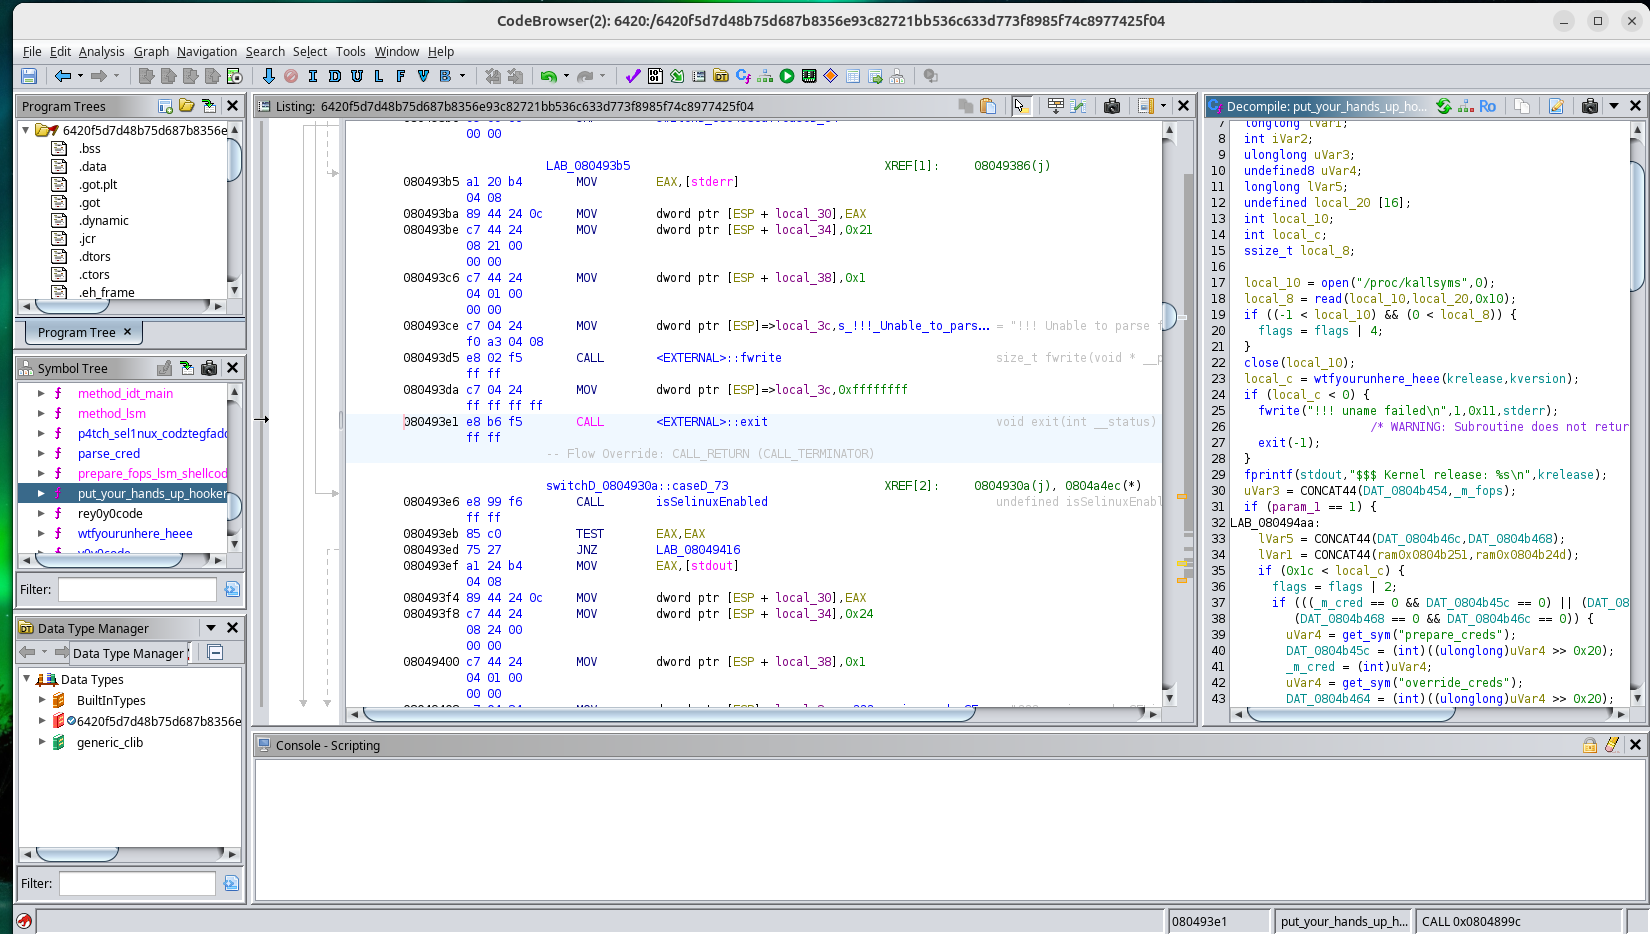
\includegraphics[width=0.6\textwidth]{img/g2.png}
\end{frame}

\begin{frame}
\frametitle{Static Analysis Using Ghidra}

\begin{itemize}
    \item \textbf{Benefits of Ghidra's Decompiled View:}
    \begin{itemize}
        \item Provides a high-level, human-readable representation of the code.
        \item Simplifies understanding of complex binaries.
    \end{itemize}
    \item \textbf{Avoid Manual Pattern Matching:}
    \begin{itemize}
        \item Eliminates the need to manually match patterns in assembly code.
        \item Speeds up the reverse engineering process.
    \end{itemize}
\end{itemize}

\centering
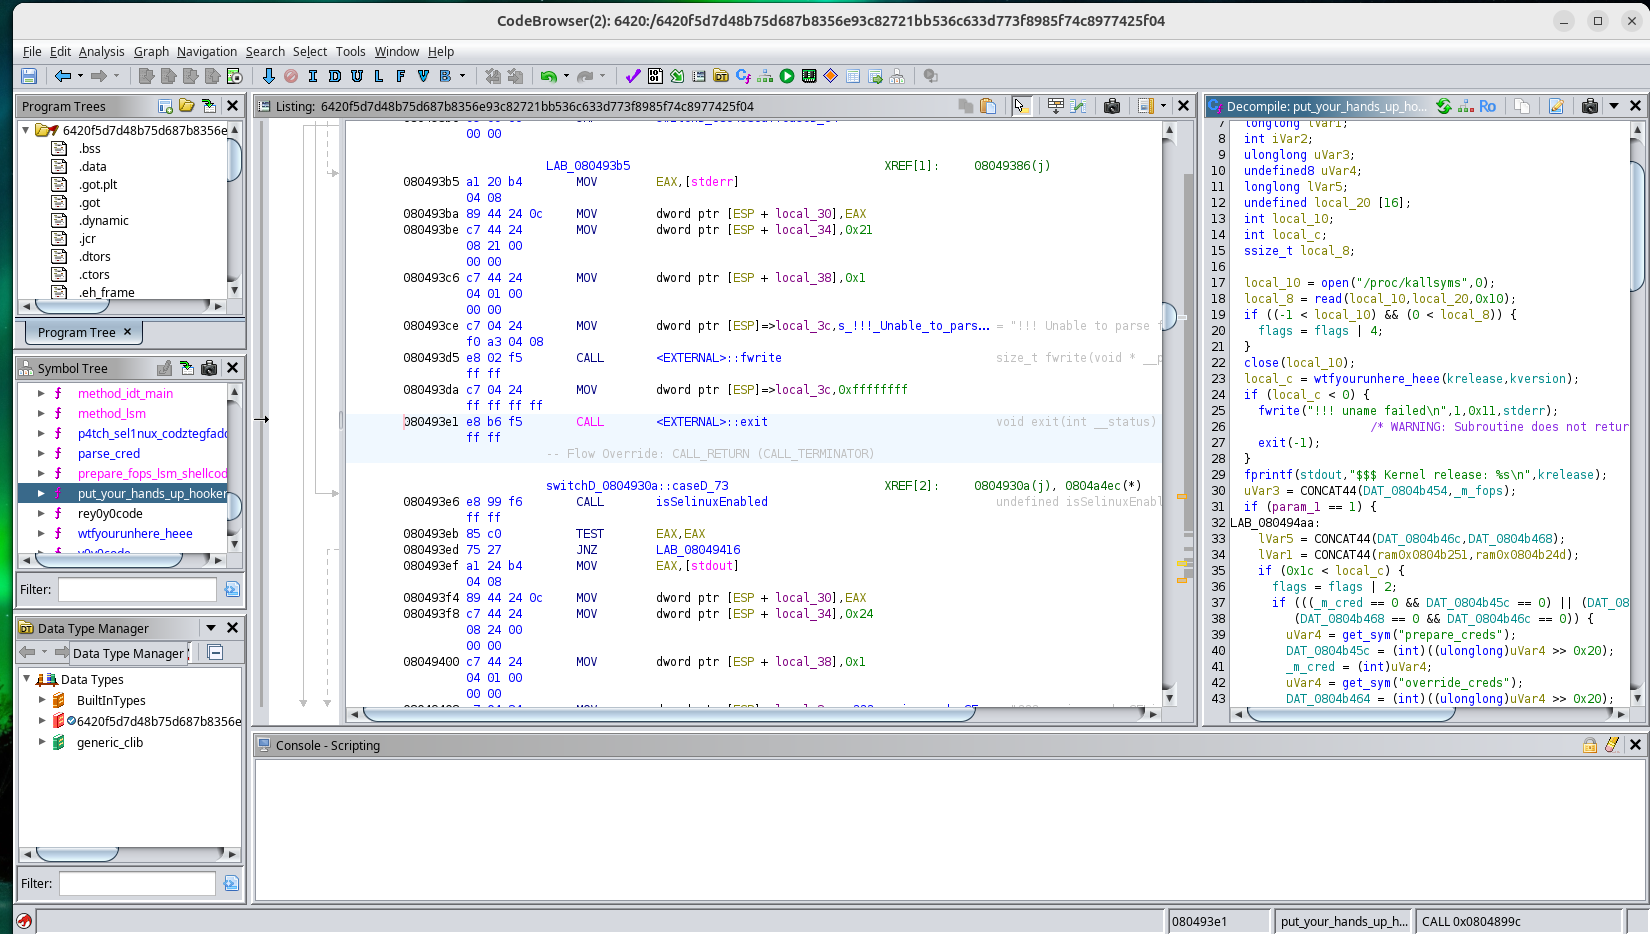
\includegraphics[width=0.6\textwidth]{img/g2.png}
\end{frame}

\begin{frame}
\frametitle{String Analysis and Cross-References in Ghidra}

\begin{itemize}
    \item Identify interesting strings, such as filenames, hardcoded paths, or error messages.
    \item Use the cross-references (Xrefs) feature to determine which functions or code sections utilize these strings.
\end{itemize}

\centering
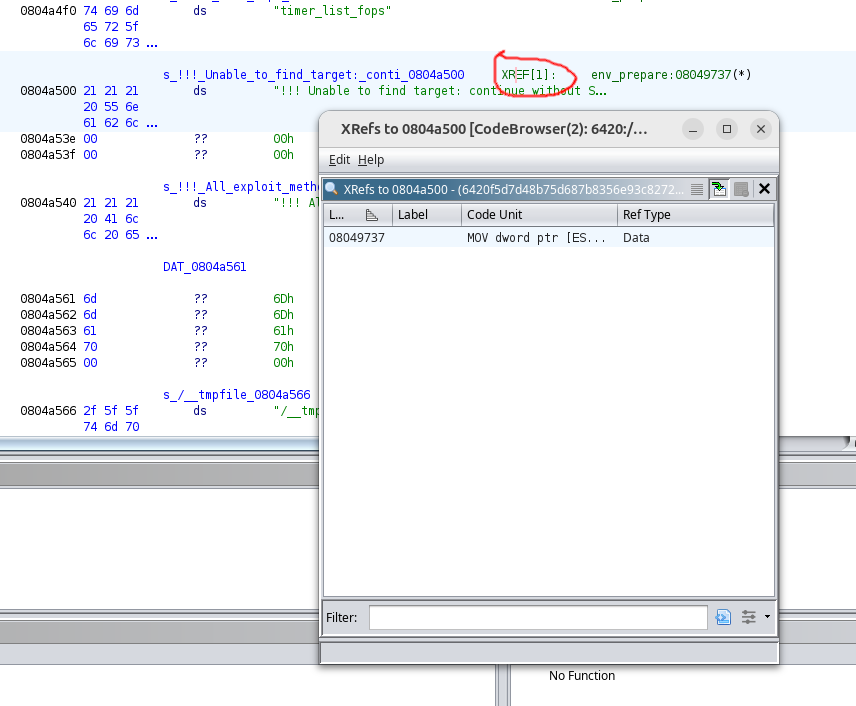
\includegraphics[width=0.6\textwidth]{img/gxref.png}
\end{frame}


\begin{frame}
\frametitle{String Analysis and Function Call Trees in Ghidra}

\begin{itemize}
    \item Certain functions are known to generate forensic artifacts, such as `fopen` and `mmap`.
    \item Locate these functions in the function call tree to identify which functions use them.
    \item Determine the artifacts that can be leveraged for detection and analysis.
\end{itemize}

\centering
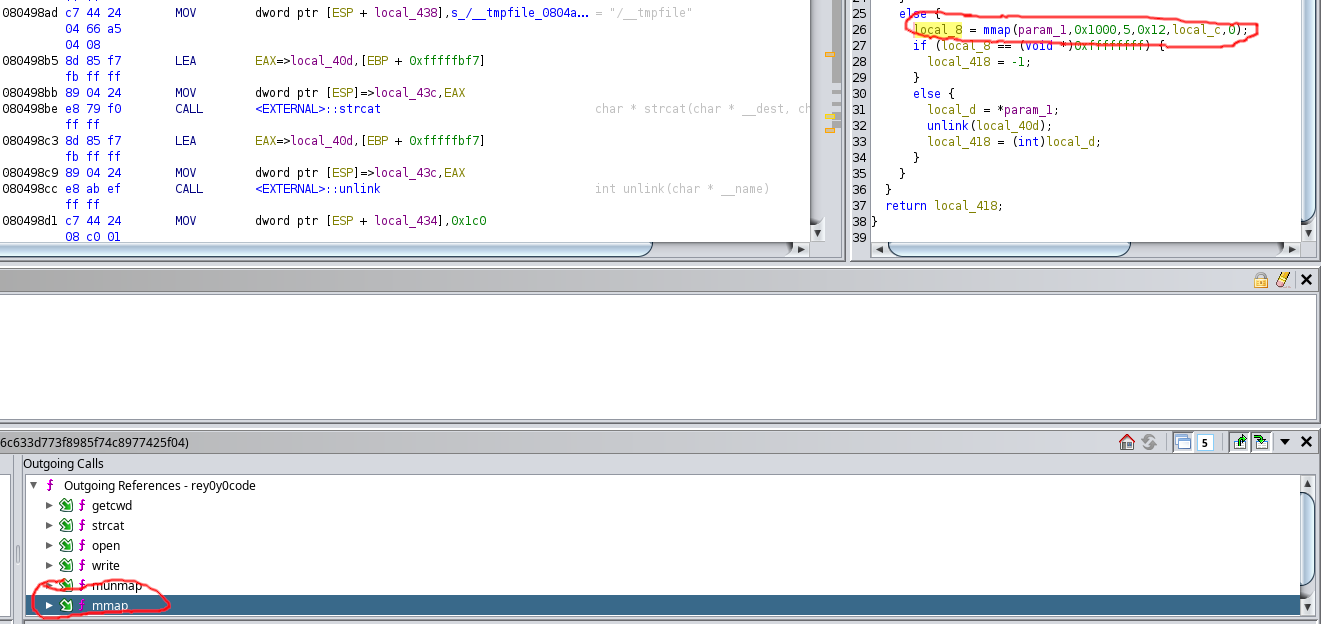
\includegraphics[width=0.6\textwidth]{img/goutcall.png}
\end{frame}


\begin{frame}
\frametitle{Static Analysis and Function Call Graphs in Ghidra}

\begin{itemize}
    \item Visual representations of function call graphs provide valuable insights into program behavior.
    \item Insights include identifying parsing activities, code execution loops, and function relationships.
\end{itemize}

\centering
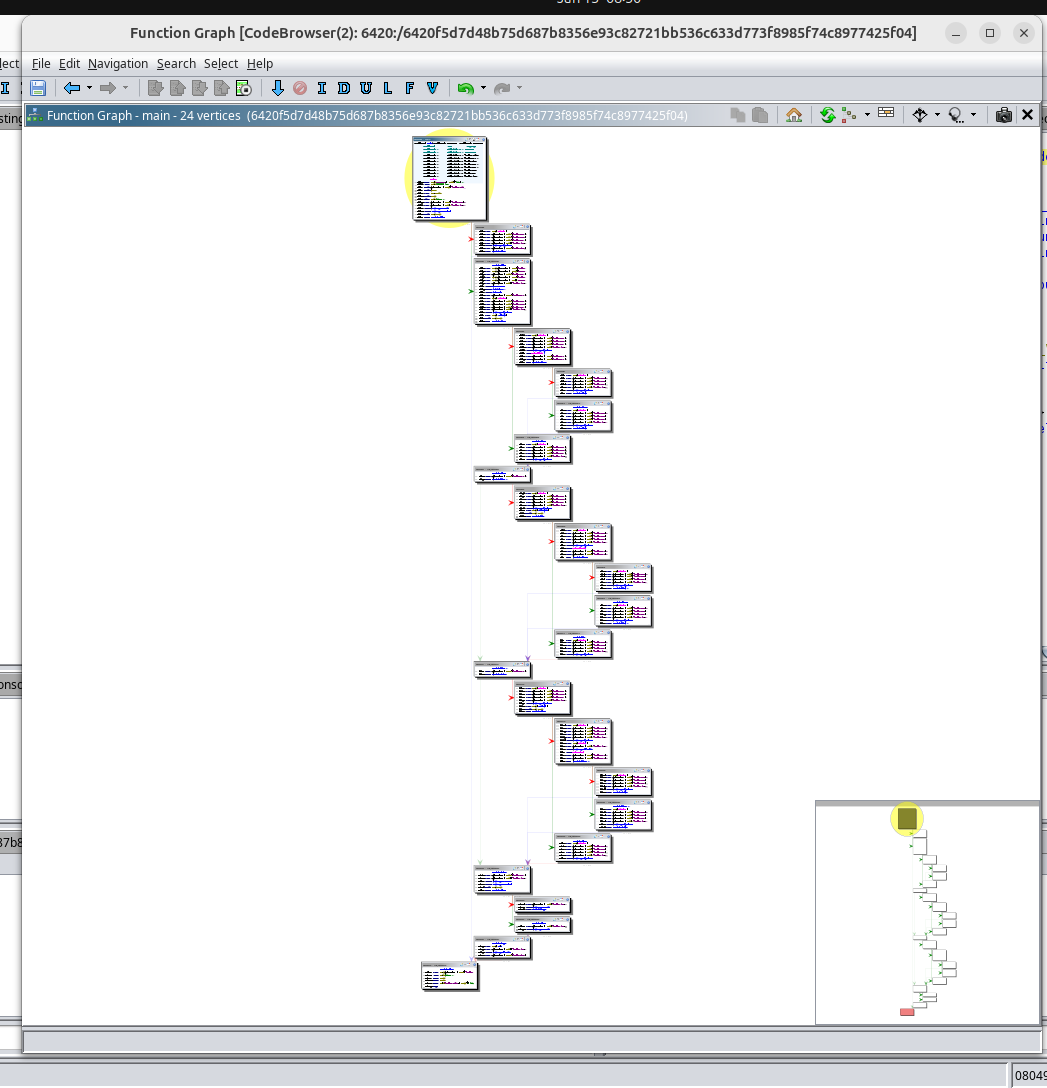
\includegraphics[width=0.6\textwidth]{img/gfctg.png}
\end{frame}

\begin{frame}
\frametitle{Core Dumps on Ubuntu}

\begin{itemize}
    \item \textbf{What is a Core Dump?}
    \begin{itemize}
        \item A core dump is a snapshot of a program's memory at the moment it crashes.
        \item Used for debugging to analyze the cause of the crash.
    \end{itemize}

    \item \textbf{Where to Find Core Dumps in Ubuntu?}
    \begin{itemize}
        \item Default location: \texttt{/var/lib/apport/coredump}.
        \item When using \texttt{systemd}, they may be in \texttt{/var/lib/systemd/coredump}.
        \item Core dumps may also be written to the program's working directory or as specified by \texttt{/proc/sys/kernel/core\_pattern}.
    \end{itemize}

    \item \textbf{Configuring Core Dumps:}
    \begin{itemize}
        \item Set unlimited size: \texttt{ulimit -c unlimited}.
        \item Check core pattern: \texttt{cat /proc/sys/kernel/core\_pattern}.
        \item Enable or configure core dumps in \texttt{/etc/security/limits.conf}.
    \end{itemize}
\end{itemize}

\end{frame}

\begin{frame}[fragile]
\frametitle{Analyzing Crash Reports}

\textbf{Problem Type:} Crash \\
\textbf{Architecture:} amd64 \\
\textbf{Crash Counter:} 1 \\
\textbf{Date:} Thu Jan 9 15:51:49 2025 \\

\textbf{Dependencies:}
\begin{itemize}
    \item adduser 3.137ubuntu1
    \item adwaita-icon-theme 46.0-1
    \item apt 2.7.14build2
    \item apt-utils 2.7.14build2
    \item at-spi2-common 2.52.0-1build1
    \item at-spi2-core 2.52.0-1build1
    \item base-passwd 3.6.3build1
    \item ca-certificates 20240203
    \item dbus 1.14.10-4ubuntu4.1
    \item dbus-bin 1.14.10-4ubuntu4.1
    \item dbus-daemon 1.14.10-4ubuntu4.1
    \item dbus-session-bus-common 1.14.10-4ubuntu4.1
    \item dbus-system-bus-common 1.14.10-4ubuntu4.1
    \item dconf-cli 0.40.0-4build2
\end{itemize}

\end{frame}

\begin{frame}[fragile]
\frametitle{Analyzing a Base64-Encoded Core Dump}

\textbf{Crash Report Details:}
\begin{itemize}
    \item \textbf{Source Package:} zoom
    \item \textbf{System Info:} Linux 6.8.0-51-generic x86\_64
    \item \textbf{User Groups:} adm, cdrom, dip, kvm, libvirt, lpadmin, plugdev, sudo, users
    \item \textbf{Core Dump Format:} Base64 Encoded
\end{itemize}

\textbf{Base64 Blob (Partial):}
\begin{verbatim}
H4sICAAAAAAC/0NvcmVEdW1wAA==
7J0HgBPV2v5nYUGaGhuiog5WLECogqJEEQVBjCiKlSy7C6y0sLsgYIsFxZ5r78Te
74169drQ2LnW2LvGjj2Wq
\end{verbatim}

\textbf{Note:} Decode the Base64 blob to retrieve the original core dump using the following command:
\begin{verbatim}
echo "H4sICAAAAAAC/0NvcmVEdW1wAA==" | base64 -d > coredump.gz
gunzip coredump.gz
\end{verbatim}

\end{frame}

\begin{frame}
\frametitle{Extracting Core Dumps from Crash Files}

\begin{itemize}
    \item Unzipping the core dump creates a file such as \texttt{\_opt\_zoom\_ZoomWebviewHost.1000.crash}.
    \item Decoding and decompressing the binary blob will produce a core dump.
\end{itemize}


\begin{block}{Extracted Core Dump Details}
\textbf{Format:} ELF 64-bit LSB core file, x86-64 \\
\textbf{Details:} SVR4-style, from \texttt{/opt/zoom/ZoomWebviewHost --type=utility --utility-sub-type=screen\_ai.mojom.Scr} \\
\textbf{User Info:} real uid: 1000, effective uid: 1000, real gid: 1000, effective gid: 1000 \\
\textbf{Exec Path:} \texttt{/opt/zoom/ZoomWebviewHost} \\
\textbf{Platform:} x86\_64
\end{block}

\textbf{Note:} Use tools like \texttt{gdb}, \texttt{readelf}, or \texttt{objdump} to analyze the extracted core dump.

\end{frame}


\begin{frame} \frametitle{dummy title 1} \end{frame}
\begin{frame} \frametitle{dummy title 2} \end{frame}
\begin{frame} \frametitle{dummy title 3} \end{frame}
\begin{frame} \frametitle{dummy title 4} \end{frame}
\begin{frame} \frametitle{dummy title 5} \end{frame}
\begin{frame} \frametitle{dummy title 6} \end{frame}
\begin{frame} \frametitle{dummy title 7} \end{frame}
\begin{frame} \frametitle{dummy title 8} \end{frame}
\begin{frame} \frametitle{dummy title 9} \end{frame}
\begin{frame} \frametitle{dummy title 10} \end{frame}
\begin{frame} \frametitle{dummy title 11} \end{frame}
\begin{frame} \frametitle{dummy title 12} \end{frame}
\begin{frame} \frametitle{dummy title 13} \end{frame}
\begin{frame} \frametitle{dummy title 14} \end{frame}
\begin{frame} \frametitle{dummy title 15} \end{frame}
\begin{frame} \frametitle{dummy title 16} \end{frame}
\begin{frame} \frametitle{dummy title 17} \end{frame}
\begin{frame} \frametitle{dummy title 18} \end{frame}
\begin{frame} \frametitle{dummy title 19} \end{frame}
\begin{frame} \frametitle{dummy title 20} \end{frame}
\begin{frame} \frametitle{dummy title 21} \end{frame}
\begin{frame} \frametitle{dummy title 22} \end{frame}
\begin{frame} \frametitle{dummy title 23} \end{frame}
\begin{frame} \frametitle{dummy title 24} \end{frame}
\begin{frame} \frametitle{dummy title 25} \end{frame}
\begin{frame} \frametitle{dummy title 26} \end{frame}
\begin{frame} \frametitle{dummy title 27} \end{frame}
\begin{frame} \frametitle{dummy title 28} \end{frame}
\begin{frame} \frametitle{dummy title 29} \end{frame}
\begin{frame} \frametitle{dummy title 30} \end{frame}
\begin{frame} \frametitle{dummy title 31} \end{frame}
\begin{frame} \frametitle{dummy title 32} \end{frame}
\begin{frame} \frametitle{dummy title 33} \end{frame}
\begin{frame} \frametitle{dummy title 34} \end{frame}
\begin{frame} \frametitle{dummy title 35} \end{frame}
\begin{frame} \frametitle{dummy title 36} \end{frame}
\begin{frame} \frametitle{dummy title 37} \end{frame}
\begin{frame} \frametitle{dummy title 38} \end{frame}
\begin{frame} \frametitle{dummy title 39} \end{frame}
\begin{frame} \frametitle{dummy title 40} \end{frame}
\begin{frame} \frametitle{dummy title 41} \end{frame}
\begin{frame} \frametitle{dummy title 42} \end{frame}
\begin{frame} \frametitle{dummy title 43} \end{frame}
\begin{frame} \frametitle{dummy title 44} \end{frame}
\begin{frame} \frametitle{dummy title 45} \end{frame}
\begin{frame} \frametitle{dummy title 46} \end{frame}
\begin{frame} \frametitle{dummy title 47} \end{frame}
\begin{frame} \frametitle{dummy title 48} \end{frame}
\begin{frame} \frametitle{dummy title 49} \end{frame}
\begin{frame} \frametitle{dummy title 50} \end{frame}

\end{document}

